Bizzabo to platforma do zarządzania wydarzeniami, która oferuje organizatorom szeroki zakres funkcji, od planowania i promocji wydarzeń po zbieranie płatności i analizę danych. Została założona w 2011 roku, od tego czasu obsłużyła ponad 90000 wydarzeń na całym świecie. Platforma jest dobrą opcją dla organizatorów wydarzeń, którzy potrzebują zaawansowanego rozwiązania do zarządzania wydarzeniami.\autocite{bizzabo}

Jedną z głównych różnic jest to, że Bizzabo jest bardziej kompleksowe niż inne platformy. Oferuje więcej funkcji i opcji konfiguracji, co może być przydatne dla organizatorów wydarzeń, którzy potrzebują bardziej elastycznego rozwiązania. 

Platforma zapewnia kompleksową organizację oraz obsługę wydarzeń w środowisku online, hybrydowym oraz tradycyjnym na żywo. Umożliwia także (\autoref{rys:biz_interfejs}) tworzenie dedykowanych stron internetowych dla danego wydarzenia, prowadzenie procesu rejestracji uczestników oraz efektywne zarządzanie płatnościami. Dodatkowo, platforma oferuje narzędzia do tworzenia i wysyłania newsletterów, a także do zarządzania marketingiem wydarzeń.

\begin{figure} [h]
    \begin{center}
    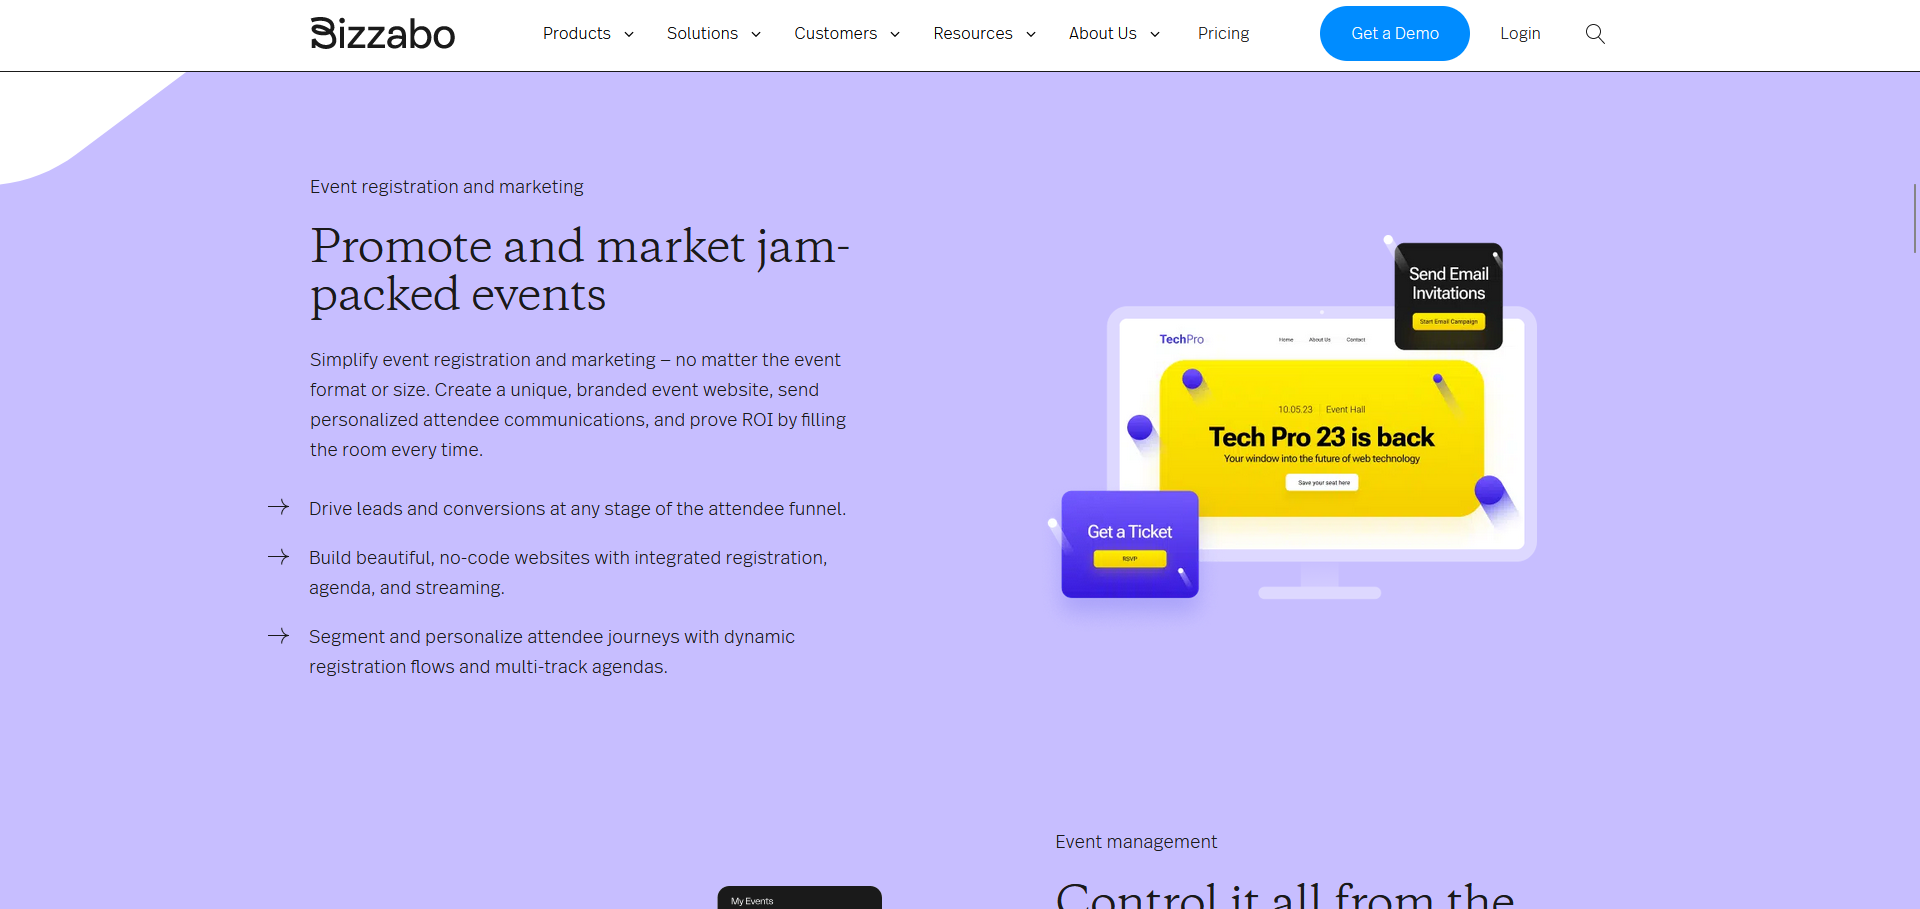
\includegraphics[scale=0.35]{imgs/solutions/bizabo.png}
    \end{center}
    \caption{Bizzabo - informacja o marketingu wydarzeń}
    \label{rys:biz_interfejs}
    \end{figure}